% Angaben zum Titel, Titelabbildung, Author und Institution




%-------------------------------------------------------
% Title
%-------------------------------------------------------
% Zwei versionen: Deutsche und Englische
\transl{%
%Title is made as a hyperlink for a fast navigation to the outline slide 
\title[\hyperlink{Outline}{CNNs}]{Implementation and Evaluation\\ of Extensions for CNNs}
}{%
\title[\hyperlink{Outline}{Logo Retrieval}]{Logo Suche in Massendaten mit Deep-Learning}
}


%-------------------------------------------------------
% Title Graphic
%-------------------------------------------------------
%
%\titlegraphic{}
%\titlegraphic{\pgfuseimage{titlegraphic}}
%
\titlegraphic{%
\centering\centerline{\ifpdf{%
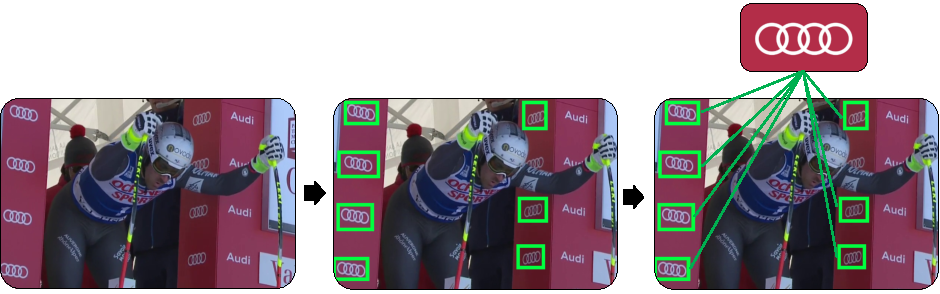
\includegraphics[height=14.5ex]{main}%
}\fi}%
}


%-------------------------------------------------------
% Author(s) / Presenter
% In eckigen Klammern Kurzversion für die Fusszeile
% (als Hyperlink zur Gliederung)
%-------------------------------------------------------
%
%
\author[\hyperlink{Outline}{Andras T\"uzk\"o}]{\textcolor{blue}{Andras T\"uzk\"o}}




%-------------------------------------------------------
% Date
% usage:   \date[short date]{date}
% Example: \date{\today} or \date[STACS 2003]{STACS Conference, 2003}.
%-------------------------------------------------------
%
\date{20. Juni 2017}


%-------------------------------------------------------
% Subtitle
%-------------------------------------------------------
%
\subtitle{Masterarbeit Abschlusspr\"asentation am \insertdate}
%\subtitle{Gespräch BAF am 29.06.2011}





%-------------------------------------------------------
% Institution(s)
%-------------------------------------------------------
%
\institute{\transl{%
%
%--------------------------------
% -   Hier englische Version    -
%--------------------------------
%
Karlsruhe Institute of Technology (KIT)\\
Institute for Anthropomatics\\
Vision and Fusion Lab (IES)
\\[2ex]
in cooperation with
\\[2ex]
Fraunhofer Institute of Optronics, System Technologies and Image Exploitation (IOSB)\\
Department Video Exploitation Systems\\
Karlsruhe, Germany%
%
%
}{%
%
%--------------------------------
% -    Hier deutsche Version    -
%--------------------------------
%
Karlsruher Institut f\"ur Technologie (KIT)\\
Institut f\"ur Anthropomatik\\
Lehrstuhl f\"ur Interaktive Echtzeitsysteme (IES)
\\[2ex]
in Kooperation mit
\\[2ex]
Fraunhofer-Institut f\"ur Optronik, Systemtechnik und Bildauswertung (IOSB)\\
\bigbreak
\small{\textbf{Betreuer:} Dipl.-Inform. Christian Herrmann, Dipl.-Inform. Daniel Manger}
}%transl
}%institute


